\section{Evaluation}\label{sec:evaluation}

This section presents our evaluation of the \sys prototype.  We implement the \numcases case studies on \sys.  We answer the following questions:
\begin{smenumerate}
\item How does \sys's performance overhead compare to eBPF, the state-of-the-art extension tool? 
\item Why does \sys impose lower runtime overhead than existing tools,?
\item How compatible is \sys with existing extension use-cases and kernel eBPF runtimes?
\end{smenumerate}

\paragraph{Experimental Setup}
We evaluate \sys running on two servers.  Server A is a dual-socket Intel Xeon Gold 5418Y Processor (24 cores, 2.00 GHz, 45 MB LLC) with 256 GB DDR5 memory.  Server B is a dual-socket Intel Xeon E5-2697-v2 processor (48 cores, 2.7 Ghz, 30 MB LLC) with 256 GB DDR3 memory.  Unless otherwise mentioned, each metric is the average of 10 trials.  We report averages using geometric mean when that is appropriate (\eg when calculating an average speedup).  We compare \sys to two baselines: the native execution on each system (native) and the performance running the extension on the linux eBPF ecosystem. 

\subsection{\sys Performance}

%\yusheng{Is the title performance correct? We also showcase the ability of \sys here.} \arq{Yep, we cover the performance tradeoffs on each use cases throughput.}

This section evaluates \sys's performance across the \numcases case studies.  In summary, we find that \sys offers significant improvement compared to eBPF, the current state-of-the-art extension framework.

\subsubsection{Deepflow}
\begin{figure}[t]
\centering
\begin{subfigure}{.23\textwidth}
  \centering
  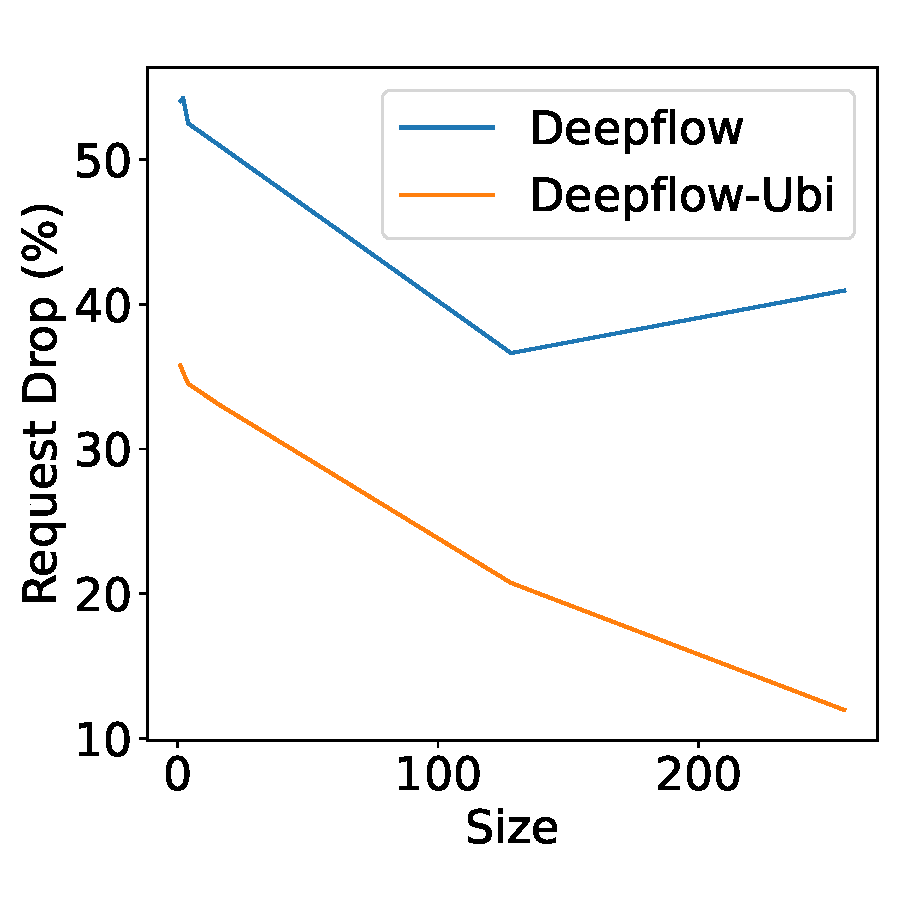
\includegraphics[width=\linewidth]{img/http-request-performance-drop.pdf}
  \caption{HTTPS}
  \label{fig:sub1}
\end{subfigure}%
\begin{subfigure}{.23\textwidth}
  \centering
  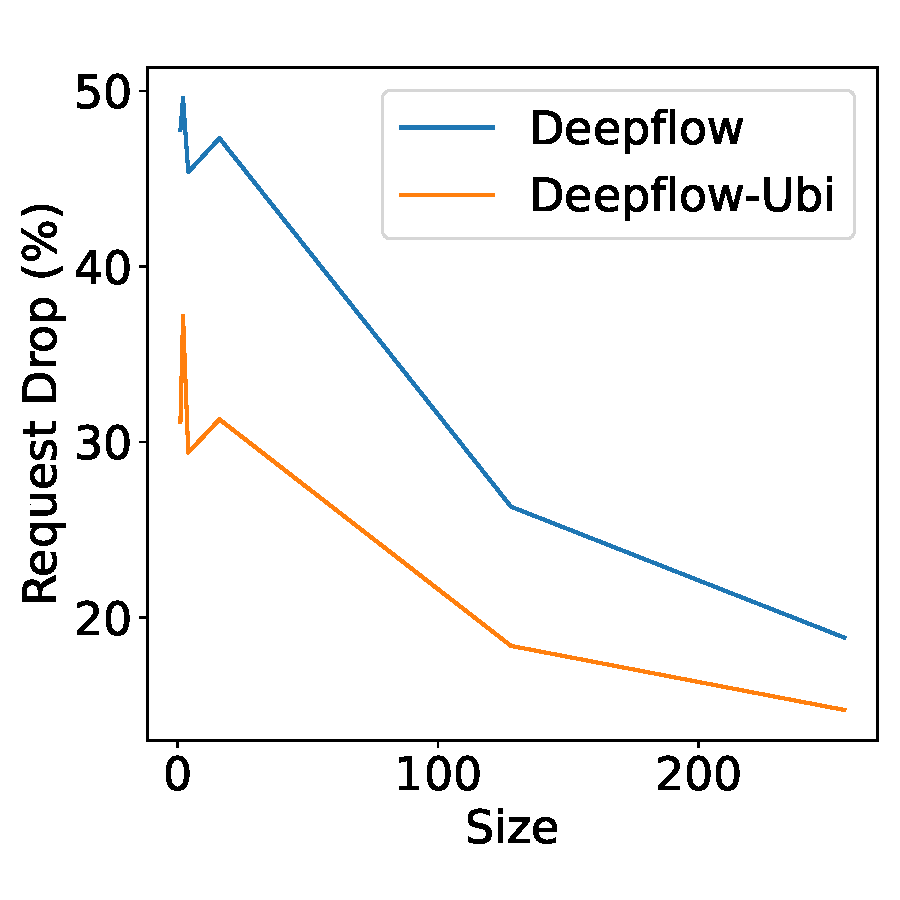
\includegraphics[width=\linewidth]{img/https-request-performance-drop.pdf}
  \caption{HTTP}
  \label{fig:sub2}
\end{subfigure}
\caption{Deepflow throughput overhead}
\label{fig:test}
\end{figure}


We deploy Deepflow on System B and use it to monitor a microservice that returns a random string for each request, implemented on a Golang server and configured to use either HTTP and HTTPS. We route traffic to the service using \texttt{wrk}, configured to use 10 threads with 500 concurrent connections for a 10-second test duration.  We execute the tests with three configurations: native microservice execution without Deepflow, Deepflow using eBPF, and Deepflow using \sys.

We measure the throughput of the microservice as we vary the size of its string response from 1KB to 256KB; \cref{fig:test} shows our results. The native microservice achieves a throughput of between 250,000 requests/second on small keys to 47,000 requests/second on large keys.  DeepFlow using eBPF imposes a significant performance penalty, reducing the throughput of the server by as much as 54\%. \sys reduces this throughput penalty by a factor of 1.5, only reaching a throughput penalty of 36\% in the worst case.

\subsubsection{Durability Tuning}
\begin{figure}[t]
\centering
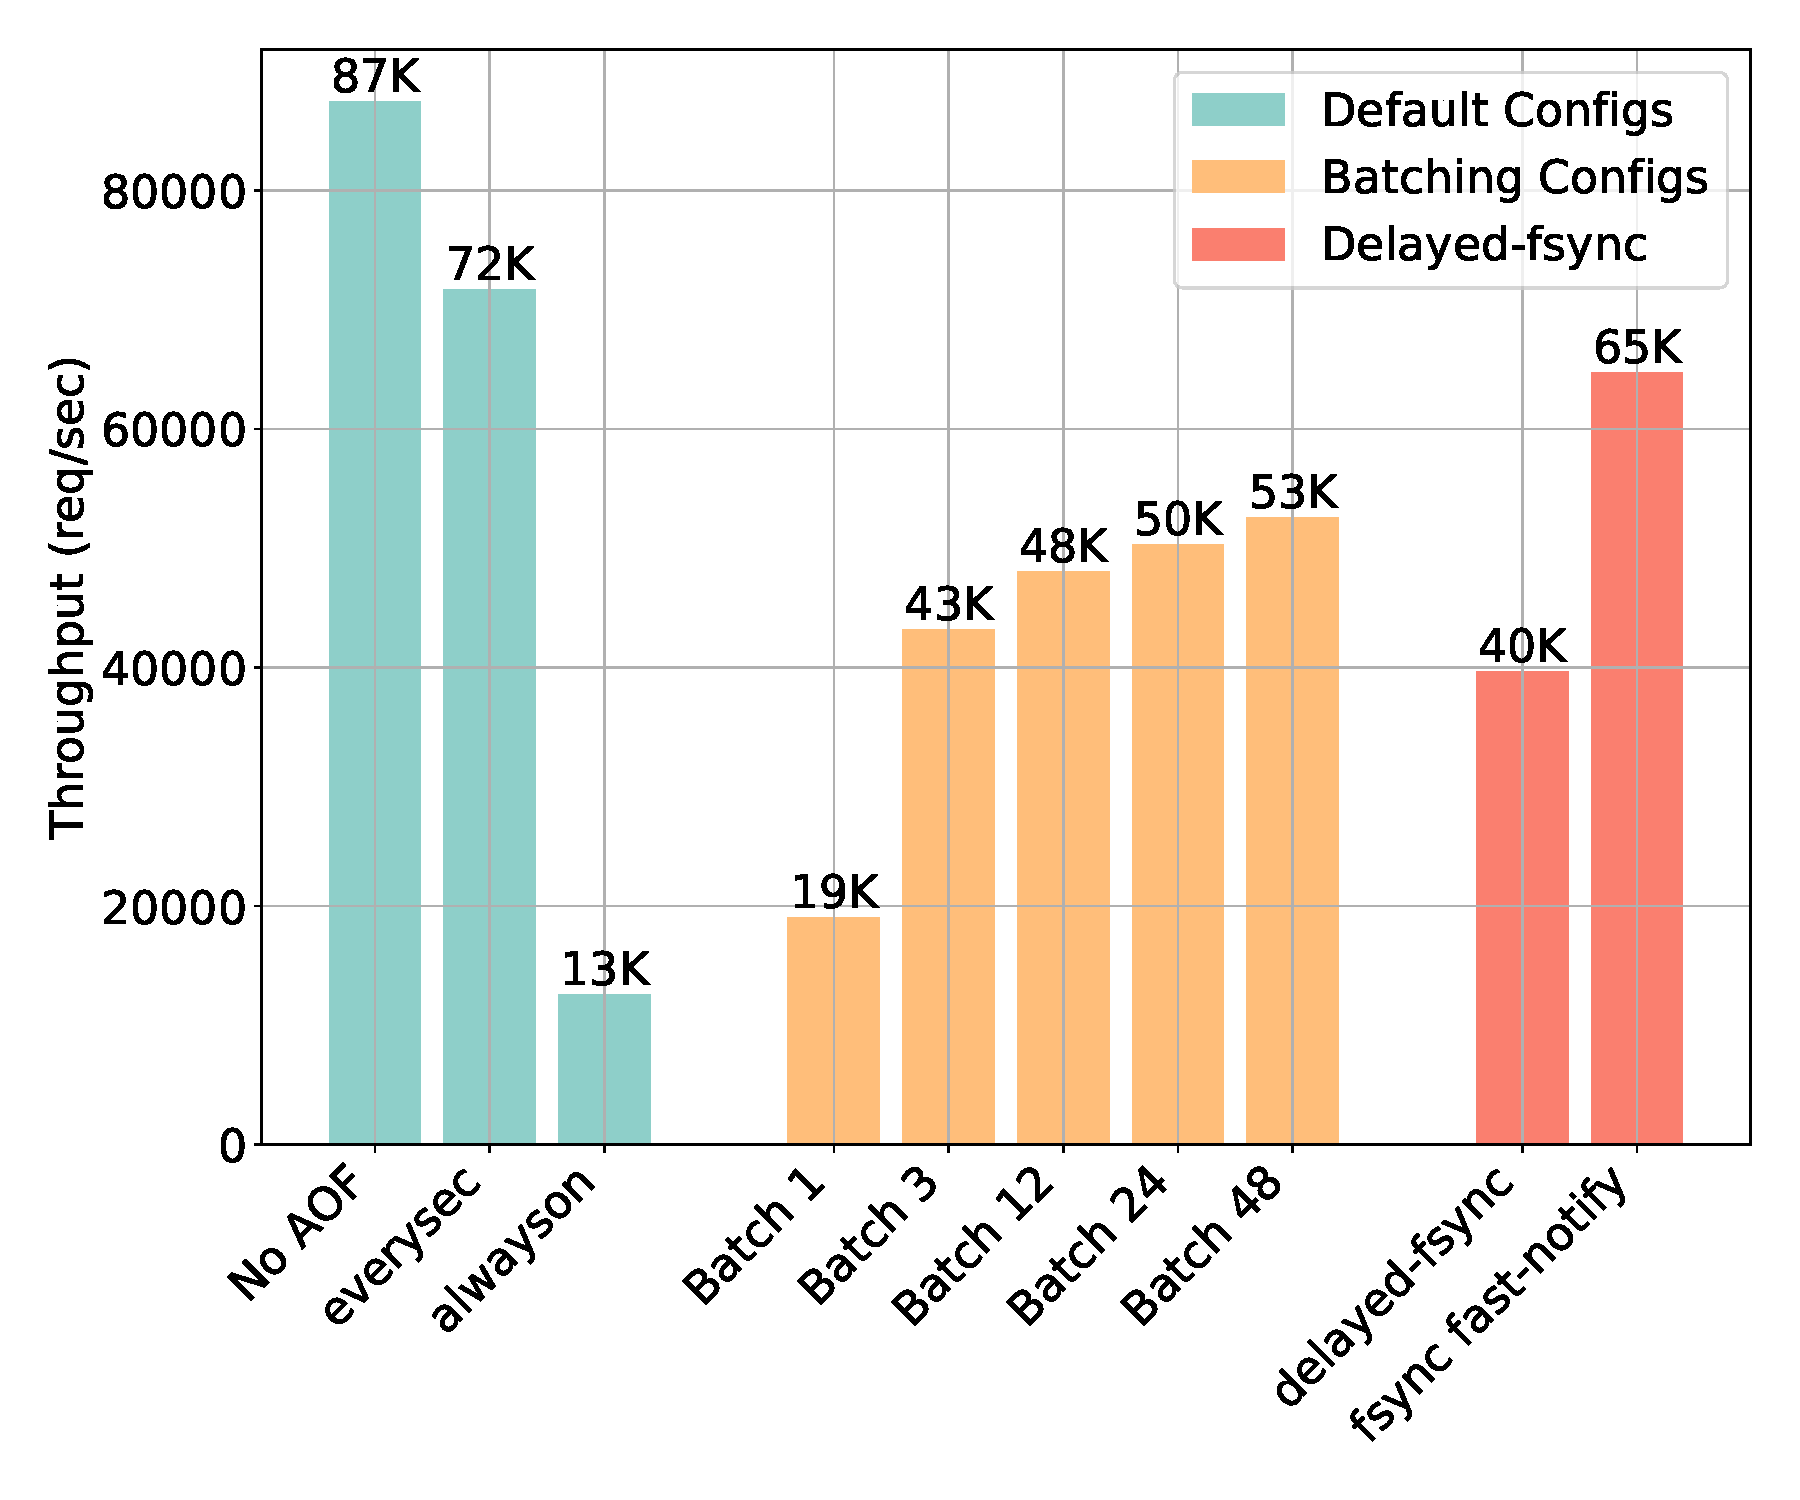
\includegraphics[width=\columnwidth]{img/redis_cluster.pdf}
\caption{Redis throughput with \sys Batch-I/O and Delayed-fsync extensions}\label{fig:redis-batch}
\end{figure}

%\yusheng{we are optimizing the color and layout.}

We evaluate the Durability Tuning use-case on System A and use redis-bench\cite{redis-bench} to send 1M set requests with 5 parallel clients and 3 byte payloads.  We execute redis with the built-in configurations (alwayson, everysec, and No AOF), varied batch sizes (1, 3, 12, 24, and 48), delayed-fsync, and delayed-fsync with the fast-notify optimization.  We configure redis with alwayson when configured to use a batching and delayed-fsync.  \Cref{fig:redis-batch} shows the throughput of each of the configurations.

The batched-I/O exposes interesting durability/performance tradeoffs.  For example, using a batch size of 48 improves redis alwayson throughput by a factor of 4.17, and incurs a modest durability cost of losing ~24 updates in the event (roughly half of the function in a batch are \texttt{write}s).  For comparison, the everysec configuration can lose 72,000 updates in the event of an untimely crash. Thus, a batch size of 48 reduces data loss relative to everysec by three orders of magnitude (2958).  Additionally, we observe that the batched-I/O implementation improves redis performance even for small batches: e.g., a batch size of 1 improves redis alwayson throughput by a factor of 1.51.

Delayed-fsync presents a powerful optimization.  On its own, delayed-fsync achieves a throughput of ~40k requests/second, which is 4.15 times larger than the redis alwayson's throughput. Adding the fast notify user-kernel interaction further accelerates redis to ~65k request/second, more than 5 times larger than redis alwayson.  In sum: delayed-fsync with fast notify is only 10\% slower than redis everysec, but it reduces the number of updates that could be lost in a crash by 5 orders of magnitude (36,000). 

\subsubsection{FUSE}
\begin{table}[t]
\centering
\footnotesize
\begin{tabular}{|l|l|l|}
\hline
\textbf{Test} & \textbf{Native (s)} & \textbf{\sys (s)} \\ \hline \hline
Passthrough, fstat & 3.65 & .176 \\ \hline
LoggedFS, fstat & 7.40 & .184 \\ \hline
LoggedFS, openat& 17.0 & 0.074 \\ \hline
Passthrough, find & 5.1 & 1.6\\\hline
\end{tabular}
\caption{FUSE operation latency.}
\label{tab:fuse}
\end{table}


We evaluate the performance improvement from using \sys to implement caching in FUSE when running on System A.  We deploy two FUSE file systems: Passthrough, which passes filesystem operations to the underlying file system directly, and LoggedFS\cite{loggerFS}, which logs all file system operations to a file before passing them to the underlying file system.  We measure the end-to-end latency of three workloads: one that issues 100000 \texttt{fstatat} calls to a file in the FUSE directory, one that issues 100000 \texttt{openat} calls to a file in the  FUSE directory, and one that uses the linux utility \texttt{find} to travel through the linux 6.7 source code directory.  
%We measure the average single syscall latency for \texttt{fstat} and \texttt{openat}, and measure the end-to-end latency for \texttt{find};   
\Cref{tab:fuse} shows the results on FUSE and with \sys{} caching.  We observe that the caching extension implemented with \sys accelerates the latency of the workloads by a factor of up to four orders of magnitude.
%\arq{I changed these units to seconds and did end-to-end latency rather than average}

\subsubsection{Sslsniff}
\begin{figure}[t]
\centering
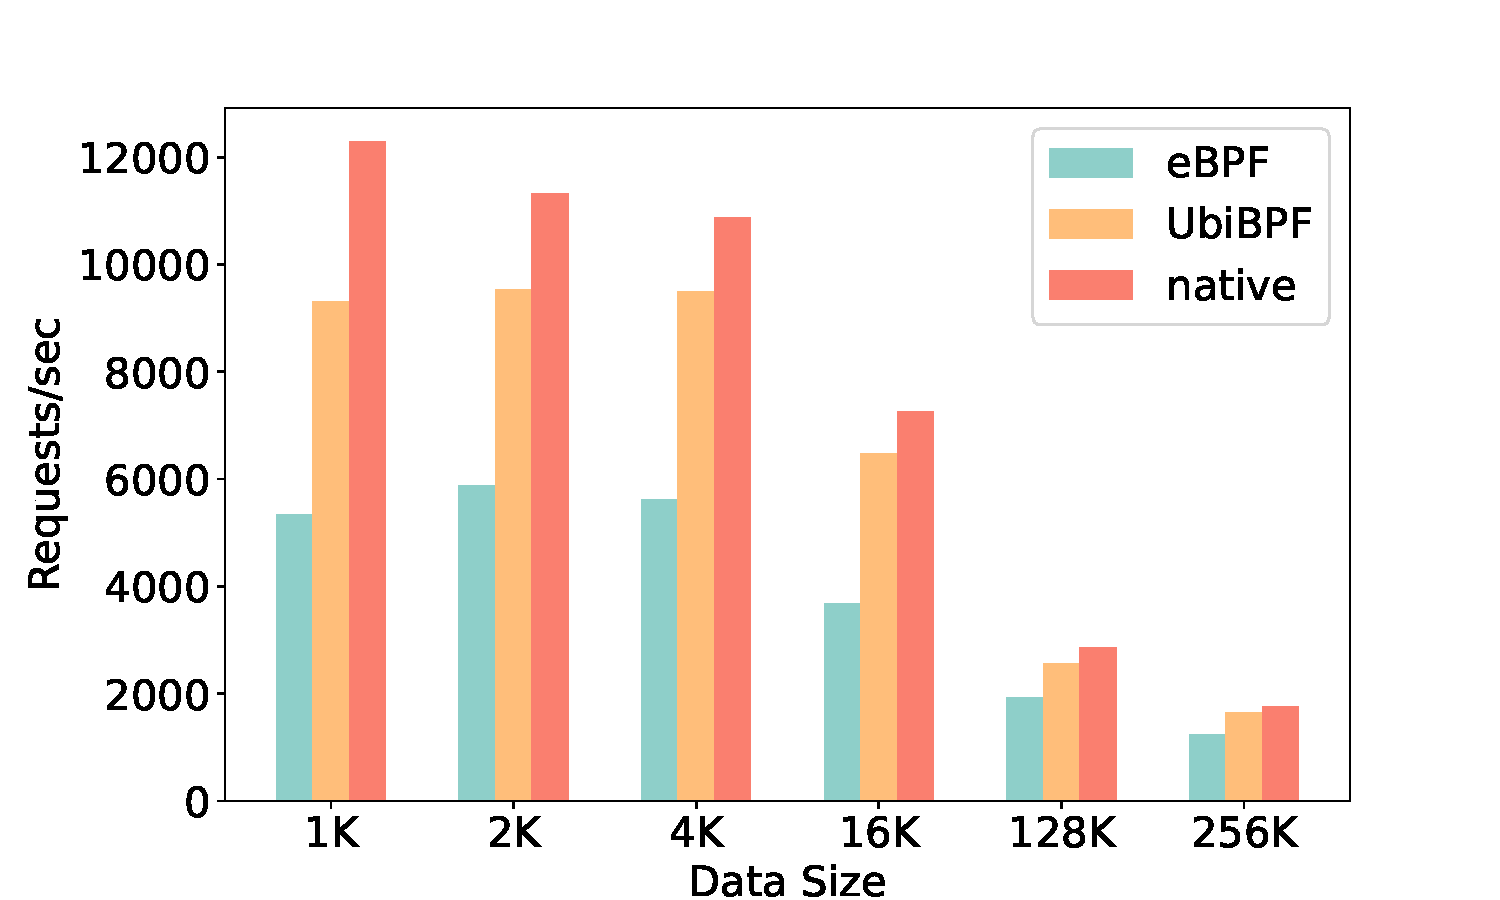
\includegraphics[width=\columnwidth]{img/ssl-nginx.pdf}
\caption{SSlsniff test with nginx}\label{fig:sslsniff}
\end{figure}

We evaluate \texttt{sslsniff} on System B when monitoring  Nginx.  We use the \texttt{wrk} benchmark, configured to use 4 threads with 512 concurrent connections for a 10 second test duration, to generate traffic.   We execute the test on three configurations: native, \texttt{sslsniff} using eBPF, and \texttt{sslsniff} using \sys.  We measure the throughput of Nginx as we vary the response size from 1K to 256KB; \cref{fig:sslsniff} shows the results.  \texttt{sslsniff} using eBPF draastically reduces Nginx performance, reducing throughput compared to native execution by a factor of up to 2.  In contrast, \sys's reduces throughput by a factor of at most 1.2.  

\subsubsection{syscount}

\begin{figure}[t]
\centering
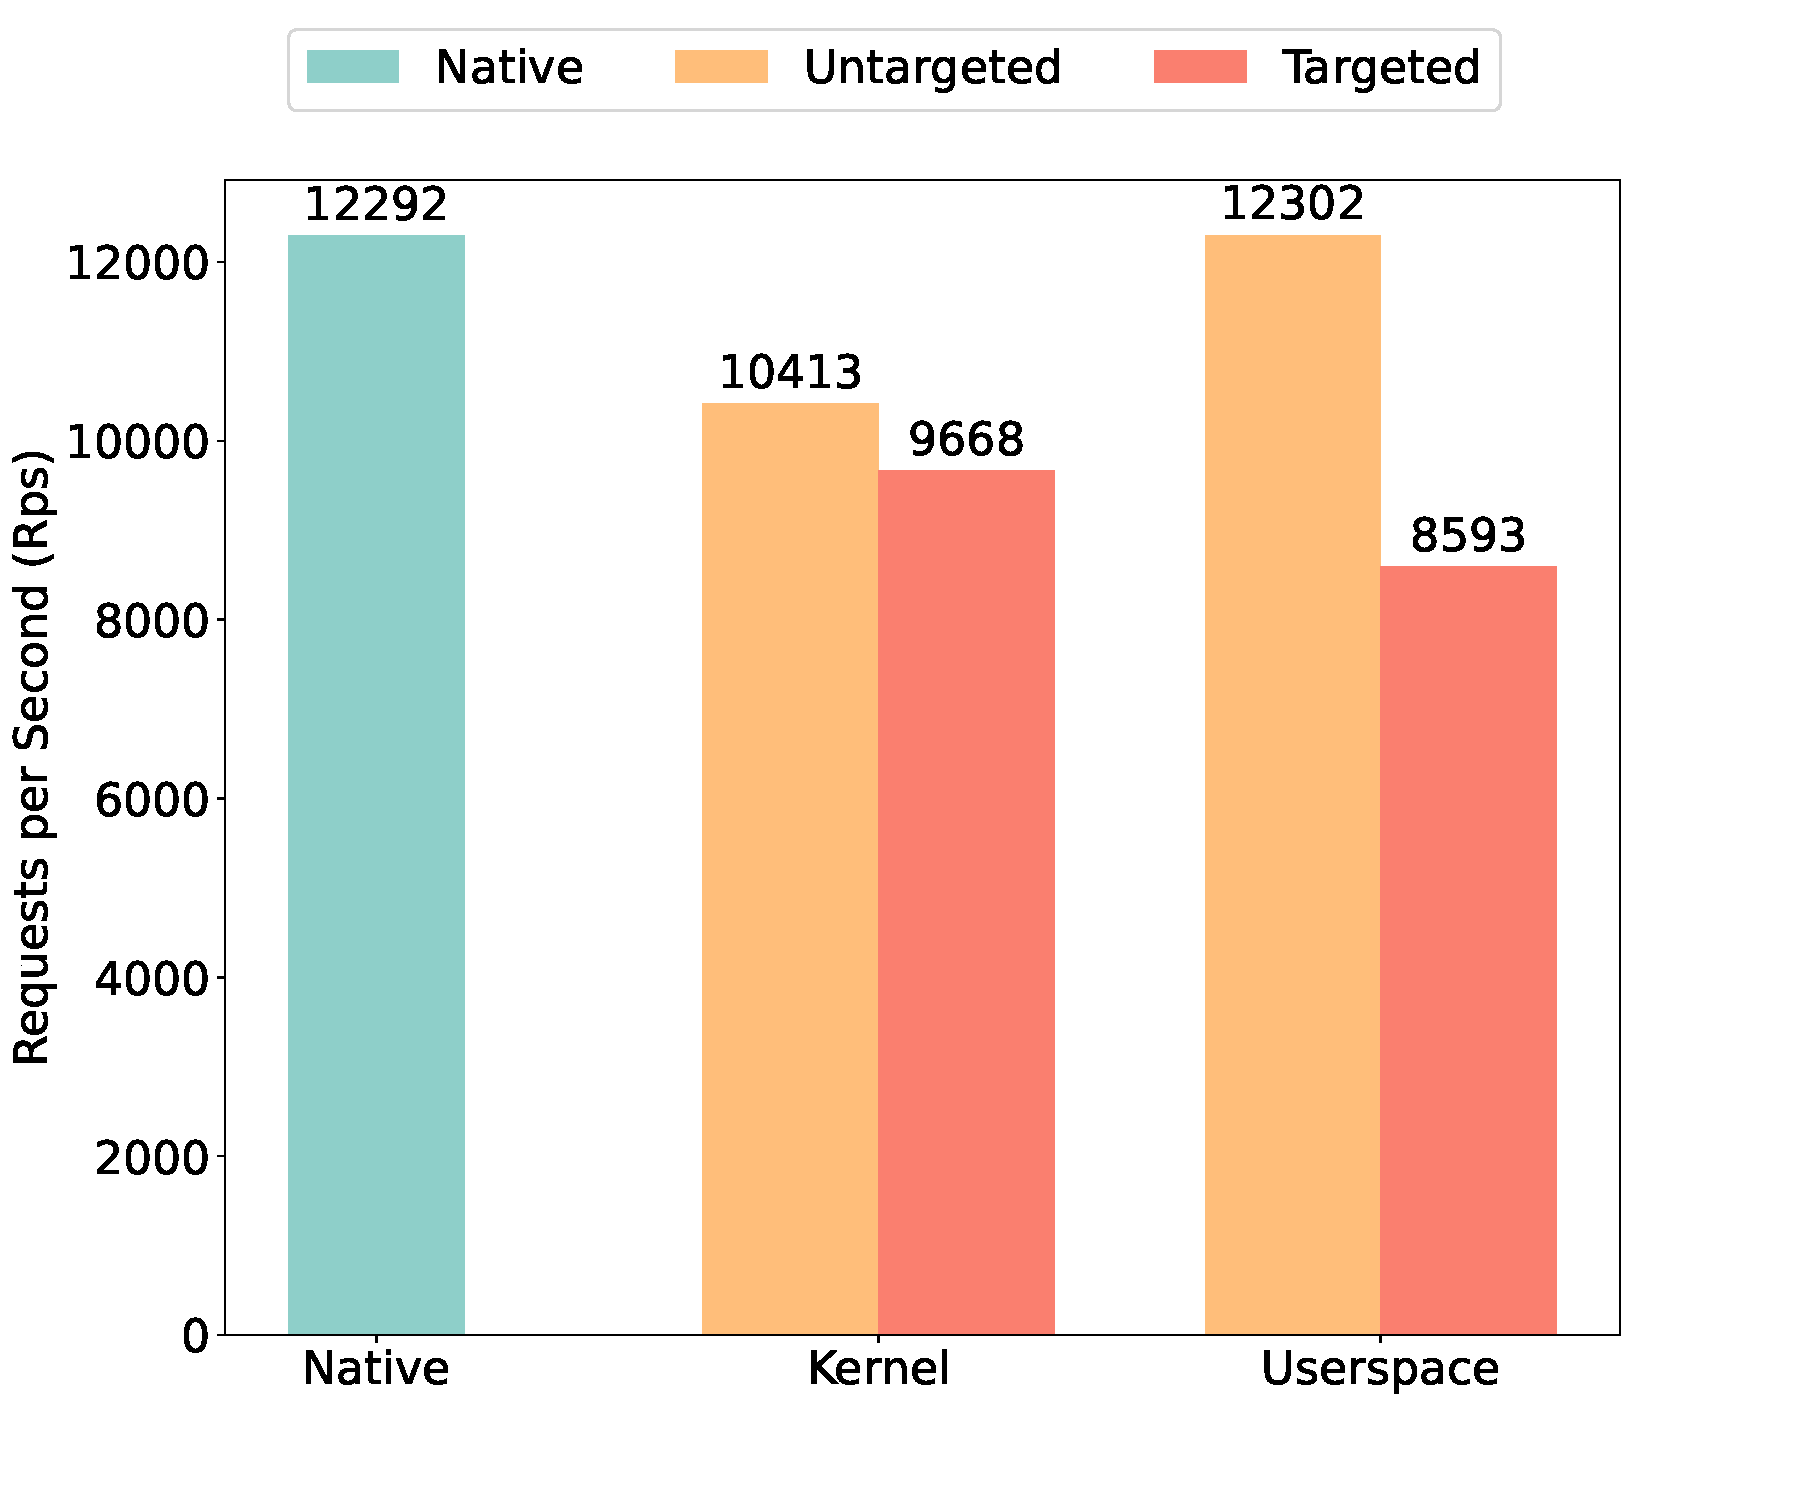
\includegraphics[width=\columnwidth]{img/syscount.pdf}
\caption{syscount test with nginx}\label{fig:sslsniff}
\end{figure}

We evaluate syscount on System B to illustrates the  \sys isolation benefits for monitoring overhead.  We deploy an Nginx server and route traffic to the server using the \texttt{wrk} benchmark, configured to use 4 threads with 512 concurrent connections for a 10-second test duration.  We measure the throughput of Nginx in five tests: (1) native Nginx, (2) syscount on the Nginx process using a kernel eBPF extension, (3) syscount on a different process using a kernel eBPF extension, (4) syscount on the Nginx process using a \sys{} userspace extension, and (5) syscount on a different process using a \sys{} userspace extension. \Cref{fig:sslsniff} shows the throughput of each of the configurations. We observe that user-mode systemcall tracing incurs more overhead than eBPF: the throughput drop from using kernel extensions is only 21.35\%, but the throughput drop from using user-mode \sys extensions is 30.09\%.  However, we also observe isolation benefits from \sys: the throughput drop from using kernel extension to monitor a different process is 15.29\%, but the throughput is not effected when using userspace \sys extension to monitor a different process. 

%\arq{Let's fix this graph!  As presented its pretty confusing, it's also missing some data. It should be a clustered bar chart.  The cluster all the way on the left shows native execution (labeled native).  The next cluster includes two bars, both of which are using kernel probes.  The first bar shows the overhead on Nginx when it is being monitored, the second bar shows the overhead of Nginx when another process is monitored.  The final cluster includes two bars, both of which are \sys.  The first bar shows the overhead on Nginx when it is moniotred with \sys, the second bar shows the overhead of Nginx when another process is monitored with \sys.} Good job

\subsubsection{Nginx Plugin}

\begin{table}[t]
\centering
\footnotesize
\begin{tabular}{|l|c|c|}
\hline
\textbf{Configuration}       & \textbf{Througput} & \textbf{Overhead} \\ \hline\hline
Native & 147000             & -               \\ \hline
\sys security    & 135000             & 8 \%              \\ \hline
Lua security   & 114000             & 22 \%              \\ \hline
Wasm security  & 106000             & 28 \%             \\ \hline
\end{tabular}
\caption{Comparison of extension approaches for Nginx}
\label{tab:nginx-plugin}
\end{table}

We evaluate the performance improvement from using \sys to extend Nginx compared to current Nginx plugins.  We deploy the security module and a tracing module in a Nginx running on System B and use \texttt{wrk} configured to use 10 worker threads with 100 concurrent connections and target a test time of 10s. We compare native Nginx execution to the security module written using \sys{} and the security module written using Nginx's Lua and WebAssembly plugins. \Cref{tab:nginx-plugin} shows the throughput of each of the configurations. \sys's extension results in an 8\% overhead compared to no filtering, whereas Lua and Wasm incur a 22\% and 28\% overhead, respectively.  Thus, \sys has 2.75x and 3.5x less overhead than Lua and Wasm.

\subsection{Microbenchmark Performance}
\begin{figure*}[t]
\centering
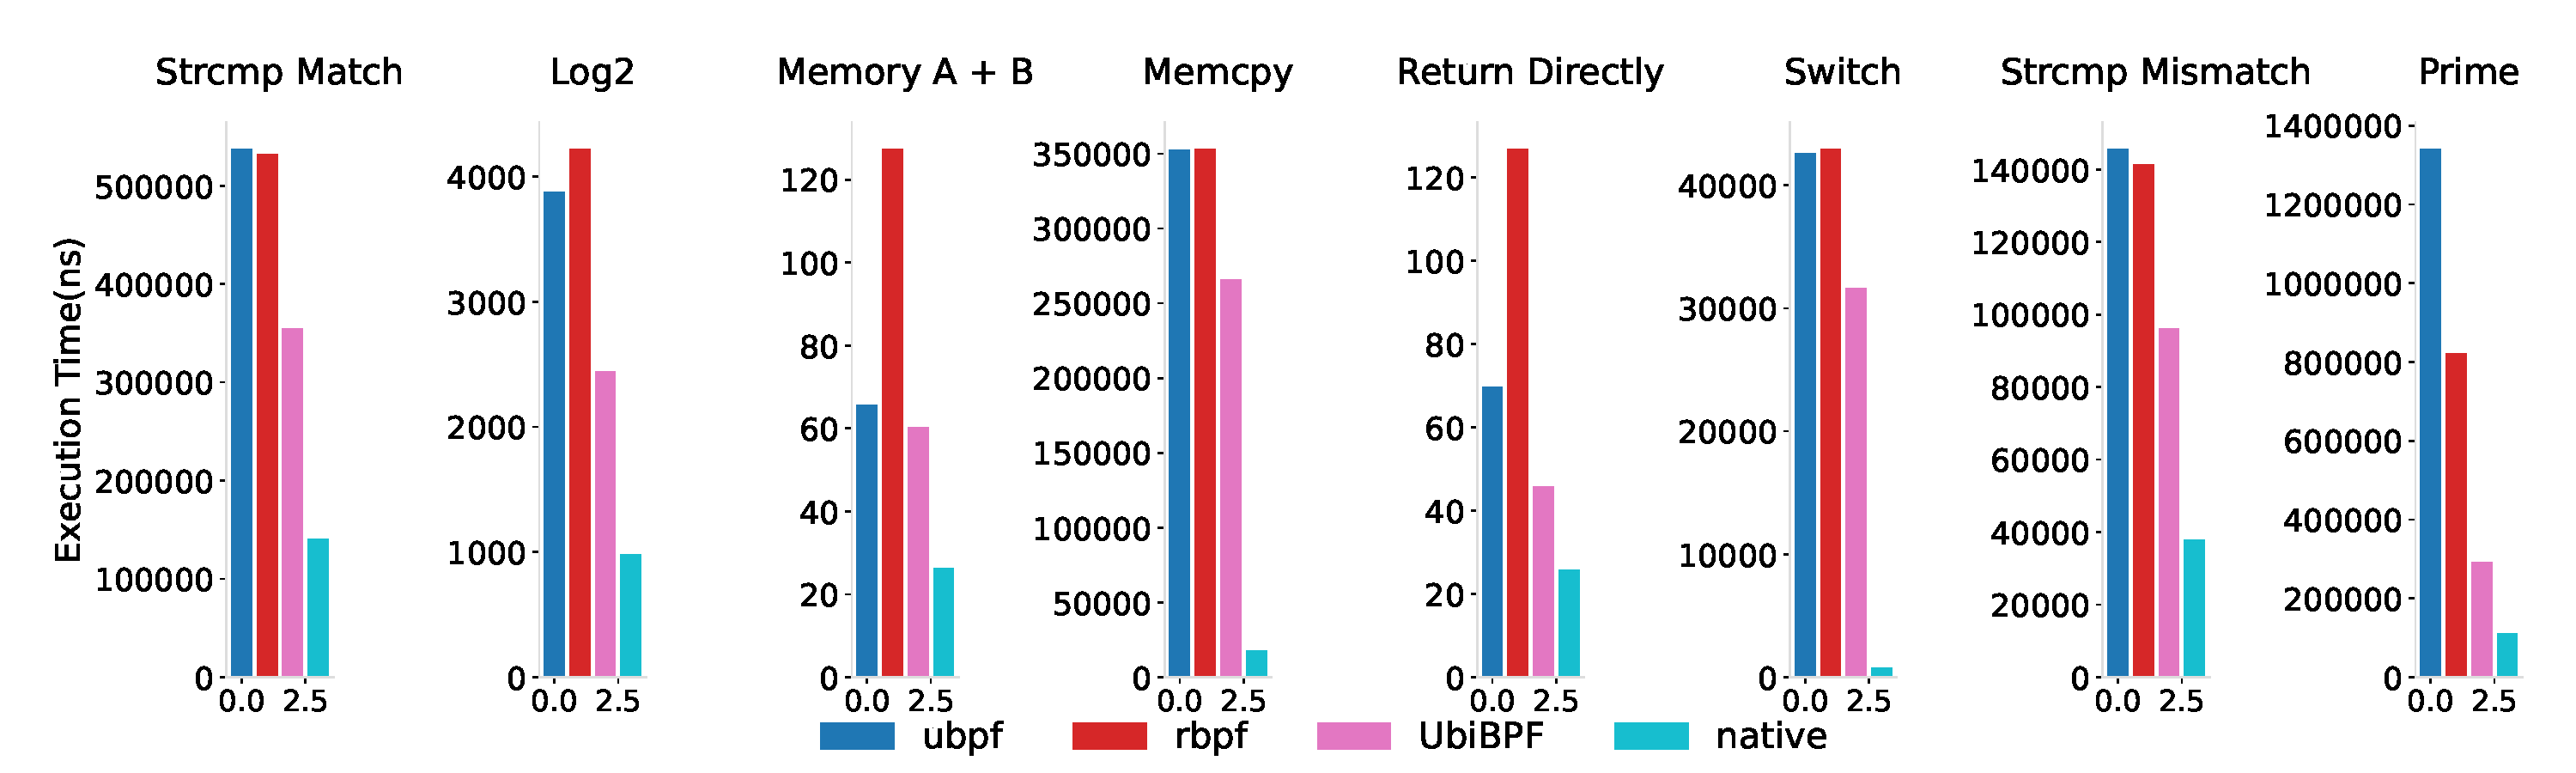
\includegraphics[width=\textwidth]{img/jit_execution_times.pdf}
\caption{Performance comparison of \sys, ubpf, rbpf, and native on microbenchmarks. \label{fig:uvm}}
\end{figure*}

We use microbenchmarks to explore \sys's efficiency.  In summary, we show that \sys's superiority comes from low per-probe latency and an efficient  eBPF bytecode execution.

\subsubsection{Probe Performance}
\begin{table}[t]
\footnotesize

    \centering
    \begin{tabular}{|c|c|c|}
        \hline
        \textbf{Probe Type} & \textbf{eBPF} (ns) & \textbf{\sys} (ns)\\
        \hline\hline
        Uprobe & 3224 & 315 \\
        Uretprobe & 3997 & 381\\
        Syscall Tracepoint & 152 & 233\\
        \hline
    \end{tabular}
    \caption{Microbenchmark comparison of \sys and eBPF.}
    \label{tab:probe_comparison}
\end{table}

We create microbenchmarks that inject and then repeatedly execute a no-op \texttt{uprobe}, \texttt{uretprobe}, and \texttt{syscall tracepoint} and execute them on system A.   \Cref{tab:probe_comparison} shows the latency of each of the probe types on eBPF and \sys.  We observe that \sys is more than an order of magnitude faster than eBPF at executing \texttt{uprobe} and \texttt{uretprobe}s, but 1.5 times slower at executing \texttt{syscall tracepoint}s.  To determine an ideal probe overhead, we statically instrument a function in our benchmark with a no-op function and observe its latency as 110 ns.  Thus, \sys's \texttt{uprobe} and \texttt{uretprobe} latencies are only a few hundred ns slower than the ideal latency. 

\subsubsection{\sys execution engine efficiency}

We evaluate the efficiency of our \sys JIT component compared to ubpf and rbpf, existing userspace eBPF virtual machines.  We write 8 micro-benchmarks, include integer heavy computation (`log2', `prime'), memory heavy workloads (`memory a+b', `memcpy'), cstring benchmarks (`strcmp match', `strcmp mismatch'), and control-flow benchmarks (`return directly', `switch').  \Cref{fig:uvm} shows the latency of each microbenchmark.  We observe that \sys is a significant improvement compared to existing eBPF runtimes (ubpf and rbpf), accelerating average benchmark latency by a factor of 1.53 and 1.72 compared to ubpf and rbpf, respectively. 

%\yusheng{9.05 is the avg of factors, it's because in memcpy and switch, native is much faster than others. 3.38 is summary all usecases, so I think we don't need to mention it here, it's hard to calc because we have so me=any different benches here.}
%3.38 mainly comes from the start and isolation delay of vm. and also the strcmp in native is using some hardware instructions to spend up.

%\arq{This graph needs a bit of help. Remove the `-jit' from ubpf and rbpf. Remove WASM from the graph (it is not helpful for the reader), and replable "<NATIVE>" to "native".  Calculate the overheads that I asked for above (the xyzs)} \arq{perfect!}

\subsubsection{\sys Load latency}
We evaluate the latency of loading an extension with \sys.  We write a test that monitors \texttt{malloc} in \texttt{libc} and measure \sys's loading latency. We load the extension into a running process and observe a 48ms load latency.  For comparison, we load the same extension using LD\_PRELOAD, a conventional technique for extending software, and observe a 30ms load latency.

\subsection{\sys Compatibility}
\begin{comment}
\begin{table}[t]
    \centering
    \begin{tabular}{|c|c|c|c|}
        \hline
        \textbf{eBPF linux} & \textbf{ubpf} & \textbf{rbpf} & \textbf{\sys} \\
        \hline\hline
        166/166 & 144/166 & 143/166 & 165/166 \\
        \hline
    \end{tabular}
    \caption{eBPF JIT pass conformance tests.}
    \label{tab:conformance}
\end{table}
\end{comment}

We evaluate the compatibility of \sys with existing eBPF full-system extensions. \sys works on all of the 17 BCC~\cite{bcc} and bpftrace~\cite{bpftrace} tools.  Also, \sys{} fails only one test in the the bpf-conformance test suite~\cite{bpfconformance}, whereas ubpf and rbpf fail 22 and 23, respectively.